%%%%%%%%%%%%%%%%%%%%%%%%%%%%%%%%%%%%%%%%%%%%%%%%%%%%%%%%%%%%%%%%%%%%%%%%%%%%%%%%%%%%%%%%%%%%%%%%%%%%%%%%%%%%%%%%%%%%%%%%%%%%%%%%%%%%%%%%%%%%%%%%%%%%%%

\UC{Visualizzazione del carrello}

\begin{figure}[H]
    \centering
    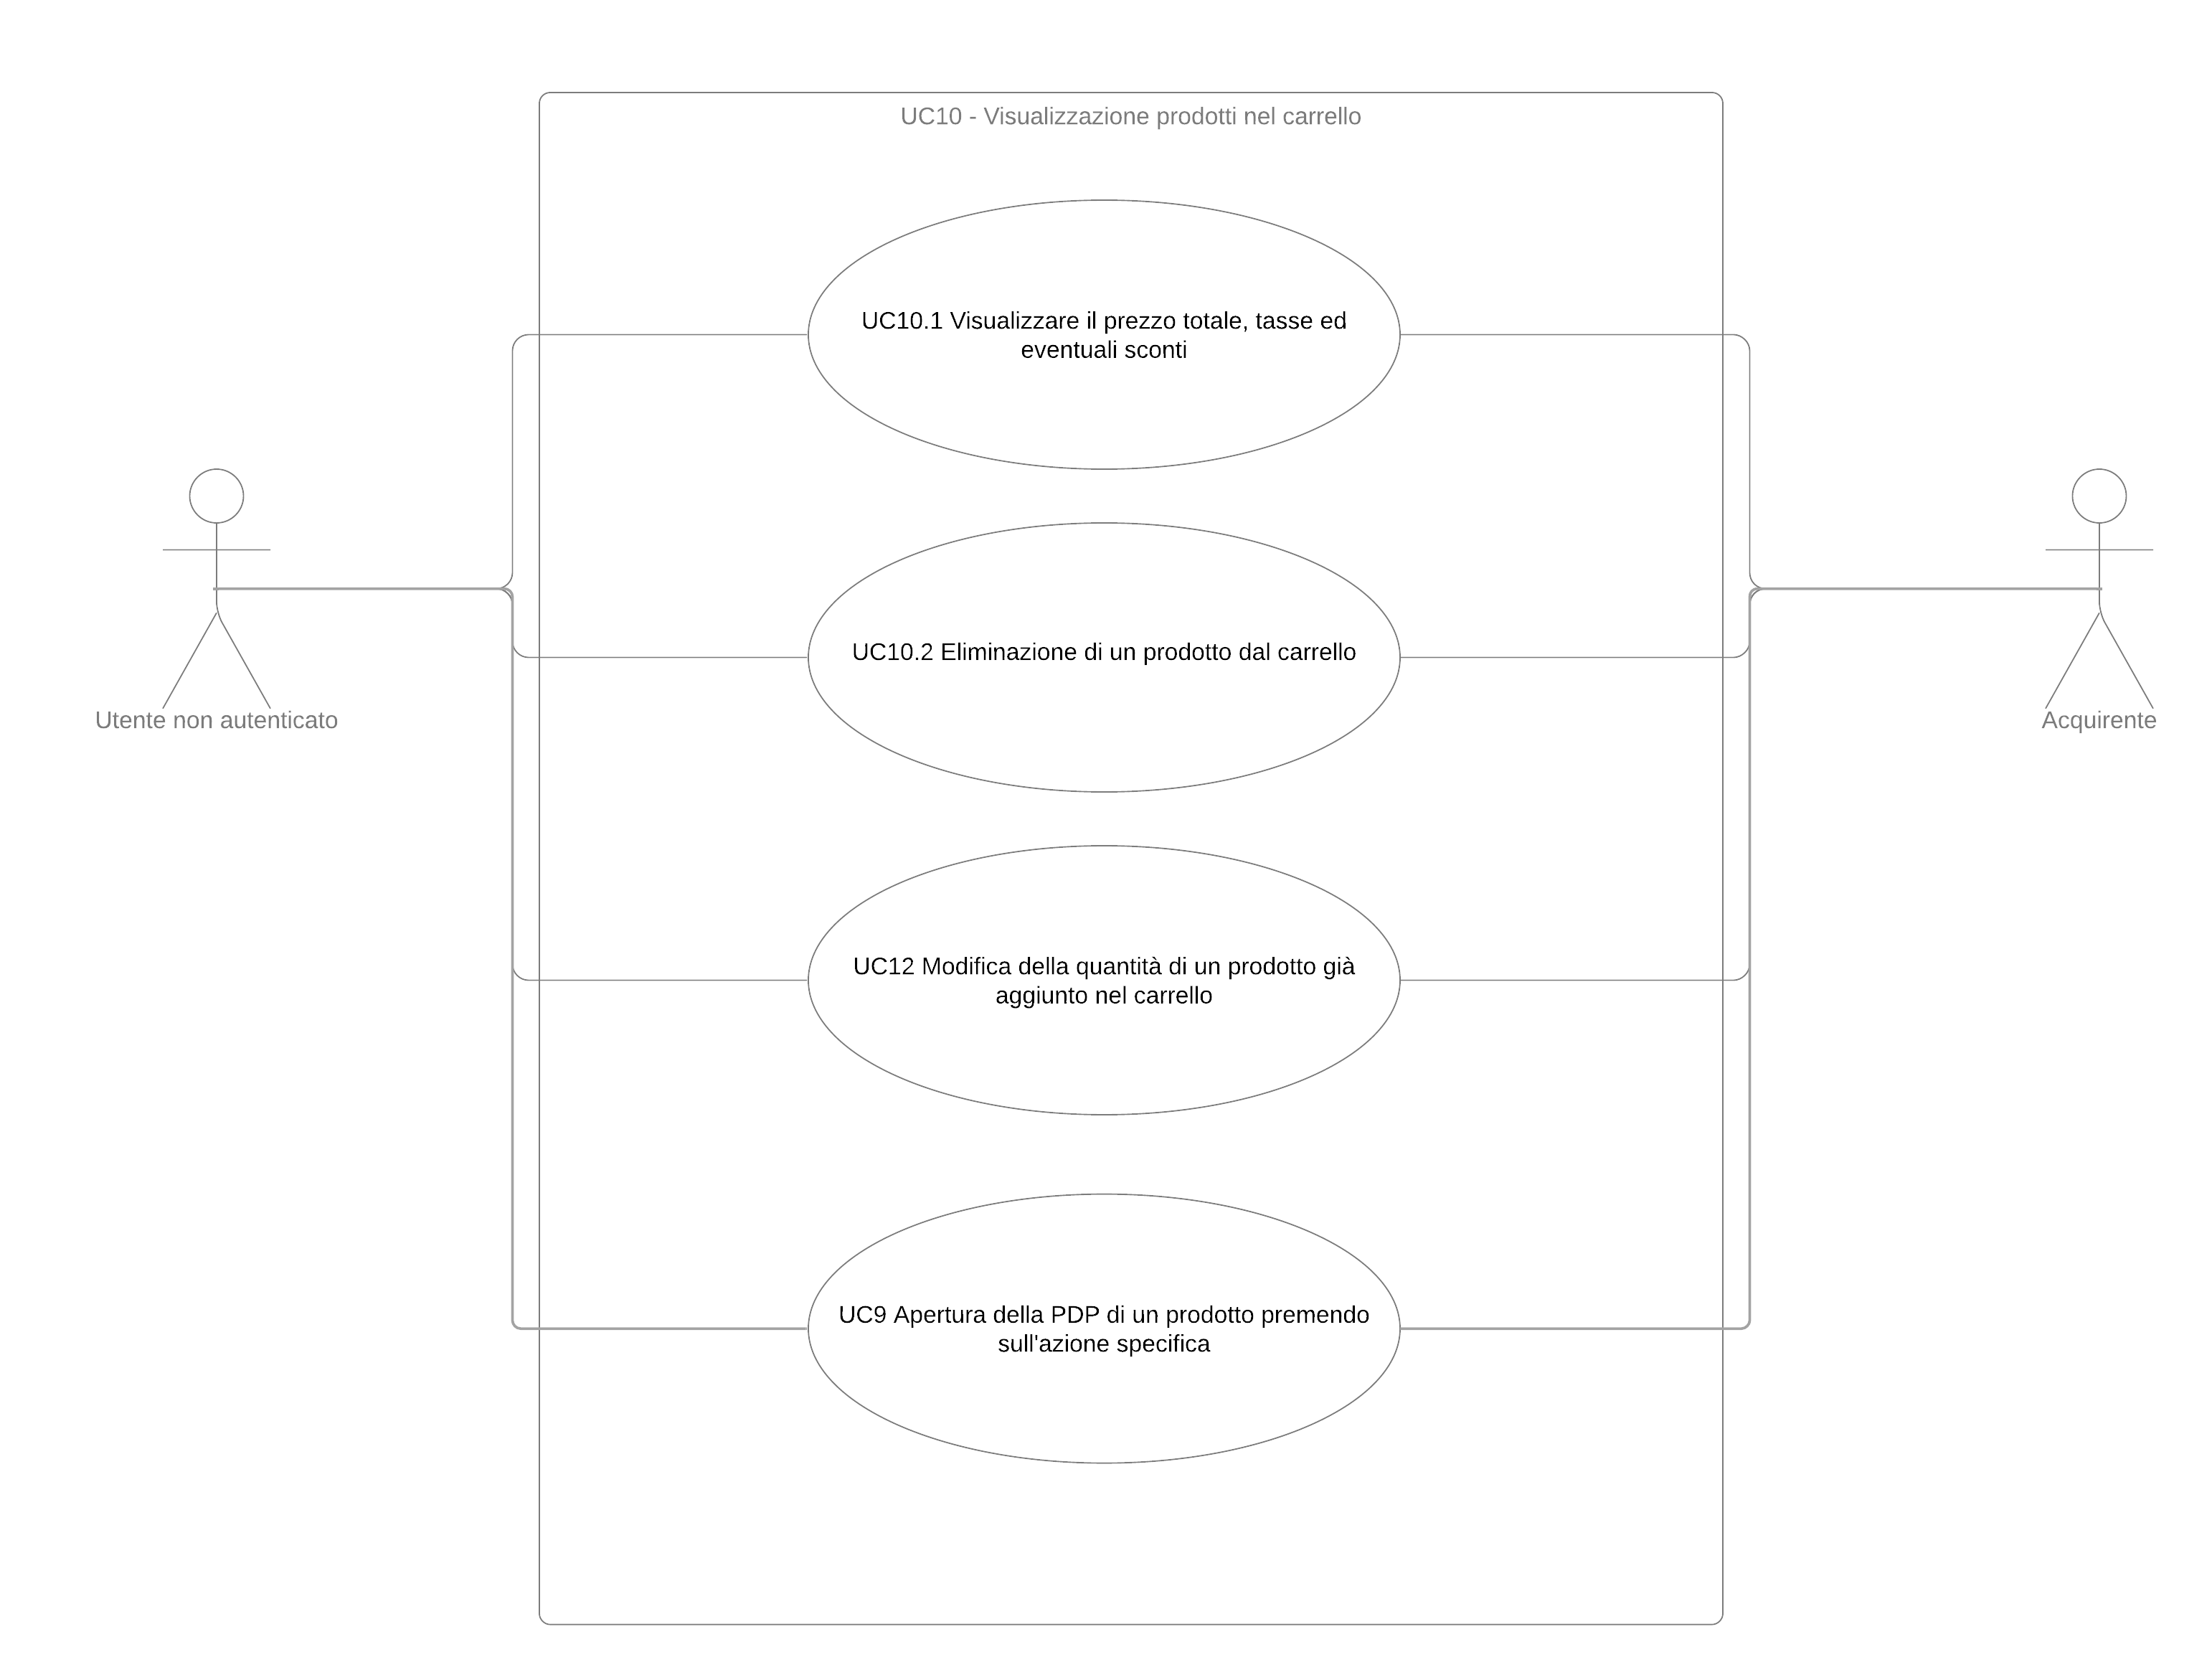
\includegraphics[width=\textwidth]{Immagini/DiagrammiUC/UC10VisualizzazioneProdottiNelCarrello.png}
    \caption{Diagramma di \actualUC: Visualizzazione prodotti nel carrello} 
    \label{fig:VisualizzazioneProdottiNelCarrello}
\end{figure}

L'utente non autenticato o l'acquirente visualizza il proprio carrello.
\begin{itemize}
    \item \textbf{Attori primari:} acquirente o utente non autenticato;
    \item \textbf{Precondizione:} l'attore si trova in una qualunque schermata della piattaforma e seleziona la funzionalità per la visualizzazione del proprio carrello;
    \item \textbf{Postcondizione:} l'attore visualizza il proprio carrello con l'elenco dei prodotti presenti;
    \item \textbf{Scenario principale:} l'attore si trova in una qualunque schermata della piattaforma e seleziona la funzionalità per la visualizzazione del proprio carrello. In seguito visualizzerà il proprio carrello dove sarà presente il prezzo totale con l'elenco dei prodotti al suo interno. Per ogni prodotto sarà visualizzato:
    \begin{itemize}
        \item Prima foto disponibile del prodotto;
        \item Nome del prodotto;
        \item Quantità inserita;
        \item Prezzo del prodotto in base alla quantità inserita e agli sconti disponibili.
    \end{itemize}
    \item \textbf{Scenari alternativi:} 
    \begin{enumerate}[label=\lett]
        \item Se non sono stati inseriti dei prodotti all'interno del carrello, verrà visualizzato il messaggio "Carrello vuoto" e sarà data la possibilità all'attore di andare alla schermata principale per iniziare gli acquisti.
    \end{enumerate}
\end{itemize}

%%%%%%%%%%%%%%%%%%%%%%%%%%%%%%%%%%%%%%%%%%%%%%%%%%%%%%%%%%%%%%%%%%%%%%%%%%%%%%%%%%%%%%%%%%%%%%%%%%%%%%%%%%%%%%%%%%%%%%%%%%%%%%%%%%%%%%%%%%%%%%%%%%%%%%

\UC{Eliminazione di un prodotto dal carrello}
L'utente non autenticato o l'acquirente può eliminare un prodotto che ha inserito nel carrello.
\begin{itemize}
    \item \textbf{Attori primari:} acquirente o utente non autenticato;
    \item \textbf{Precondizione:} l'attore è nella pagina del carrello e ha inserito almeno un prodotto;
    \item \textbf{Postcondizione:} l'attore ha rimosso totalmente il prodotto dal carrello;
    \item \textbf{Scenario principale:} l'attore non vuole più ordinare un prodotto che ha aggiunto nel carrello per questo seleziona la funzionalità di eliminazione del prodotto dal carrello, il prodotto viene quindi rimosso totalmente dal carrello.
\end{itemize}

%%%%%%%%%%%%%%%%%%%%%%%%%%%%%%%%%%%%%%%%%%%%%%%%%%%%%%%%%%%%%%%%%%%%%%%%%%%%%%%%%%%%%%%%%%%%%%%%%%%%%%%%%%%%%%%%%%%%%%%%%%%%%%%%%%%%%%%%%%%%%%%%%%%%%%

\UC{Modifica della quantità di un prodotto nel carrello}
L'utente non autenticato o l'acquirente modifica la quantità di un prodotto già nel carrello.
\begin{itemize}
    \item \textbf{Attori primari:} acquirente o utente non autenticato;
    \item \textbf{Precondizione:} l'attore è nella pagina del carrello dove ha inserito almeno un prodotto e ha selezionato la funzionalità di modifica della quantità di un prodotto;
    \item \textbf{Postcondizione:} la quantità del prodotto selezionato è stata modificata;
    \item \textbf{Scenario principale:} l'attore è nella pagina del carrello dove ha inserito almeno un prodotto e ha selezionato la funzionalità di modifica della quantità di un prodotto. In seguito la quantità di quel prodotto selezionato verrà modificata.
    \item \textbf{Estensioni:}
    \begin{enumerate}[label=\lett]
        \item L'attore modifica la quantità con una minore o uguale a zero. In questo caso:
        \begin{itemize}
            \item (UC) - Viene visualizzato il messaggio d'errore quantità del prodotto non valida;
            \item Verrà impedita la modifica della quantità nel carrello.
        \end{itemize}
    \end{enumerate}
\end{itemize}

%%%%%%%%%%%%%%%%%%%%%%%%%%%%%%%%%%%%%%%%%%%%%%%%%%%%%%%%%%%%%%%%%%%%%%%%%%%%%%%%%%%%%%%%%%%%%%%%%%%%%%%%%%%%%%%%%%%%%%%%%%%%%%%%%%%%%%%%%%%%%%%%%%%%%%
